\documentclass[13pt]{article}
\usepackage[utf8]{inputenc}
\usepackage[margin=2cm]{geometry}
\usepackage{graphicx}
\usepackage{xcolor}
\usepackage{hyperref}

\title{EcoCTD User Manual}
\author{Mathieu Dever, Mara Freilich, and Jing He}
\date{March 2019}

\newcommand{\ruskin}{\textit{RUSKIN }}
\begin{document}

\maketitle

\begin{abstract}
    This very informal document provides information on how to configure, operate, and download data from the EcoCTD probe. It requires the \ruskin software distributed by RBR. In a nutshell, what you need to know is:
    \begin{enumerate}
        \item Practice assembling/disassembling the housing
        \item Double-check that UCTD coupling piece is secure
        \item Don't forget to take sensor caps OFF and turn EcoCTD ON before deploying (seems trivial, but you'd be surprised...)
        \item NEVER GO DEEPER THAN \textbf{500 m} (about 2 min free fall)
        \item On recovery, make sure you have enough line out so a wave trough doesn't send the EcoCTD flying into the ship's stern.
        \item Protect the sensors at all time (use caps!) - except during deployment (obviously!).
    \end{enumerate}
    
    This was written quickly and poorly, but nevertheless contains important information you need to know before operating the EcoCTD.
\end{abstract}

\vfill
\hline 
\tableofcontents
\hline 

\pagebreak
\section{Instrument setup}

\subsection{Assembling the housing}
%{\it by Mara Freilich} \\ \\
Assembling and disassembling the EcoCTD requires some practice. Make sure you take the time to do it a few times before boarding the ship. You can refer to the engineering drawing below to see how the EcoCTD should be assembled. Be patient and gentle, this often takes many tries but you only have to do it once if all goes well. Always be mindful of the probes while manipulating them. The conductivity cell can easily be bent or broken, creating a leak, especially while installing the weight collars. Both the oxygen sensor and ECOPuck should be carefully handled to not be scratched. Place a protective cap on the sensors at all time.
\begin{enumerate}
    \item Attach two clamps to the RBR concerto CTD and logger. These clamps attach tightly onto the logger and screw onto the housing in order to attach the housing to the logger. The key difficulty at this step is that the clamps need to be aligned such that the housing can screw into both clamps.
    \begin{enumerate}
        \item Fasten the lower clamp above CTD and below the external ports. This clamp should slide on from below.
\begin{figure}
    \centering
    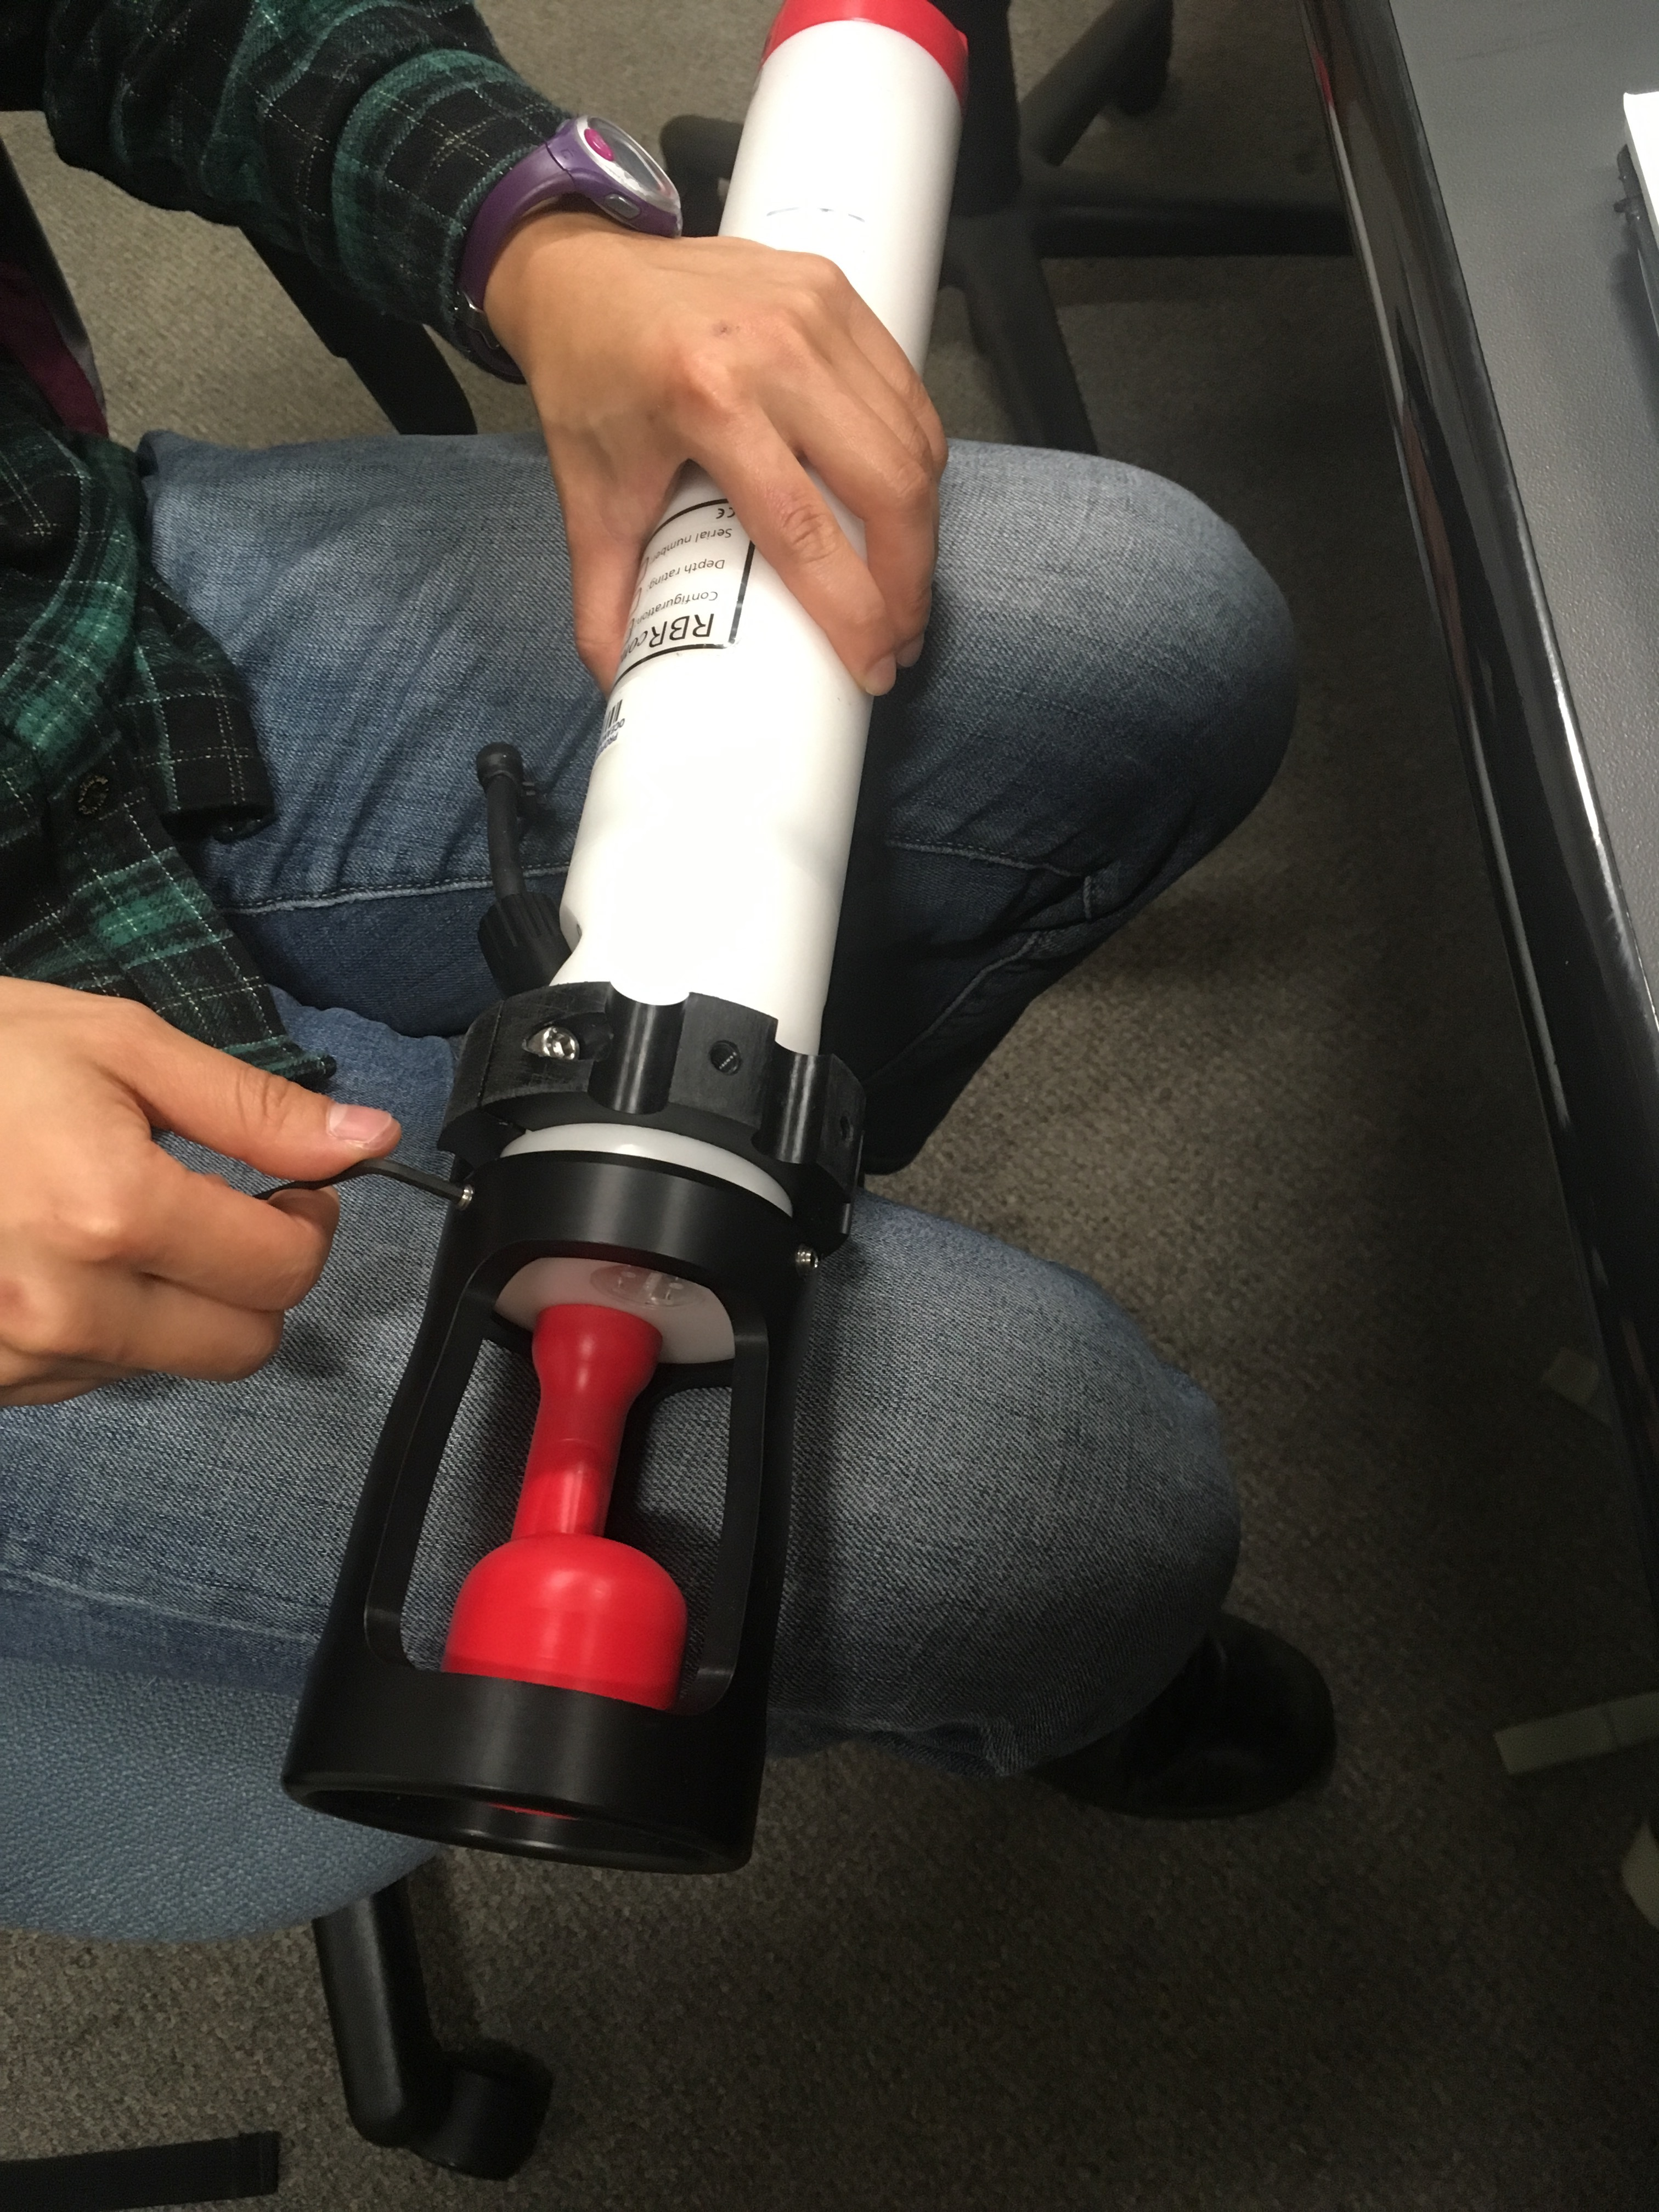
\includegraphics[width = 0.5\textwidth]{IMG_1639.JPG}
    \caption{Fastening the guard onto the CTD. The lower clamp is already attached}
    \label{fig:assemble1}
\end{figure}
        \item Fasten the guard to protect the CTD probe (Figure \ref{fig:assemble1})
        \item Fasten the upper clamp onto the CTD and logger. This clamp should slide on from above (Figure \ref{fig:assemble2}).
\begin{figure}
    \centering
    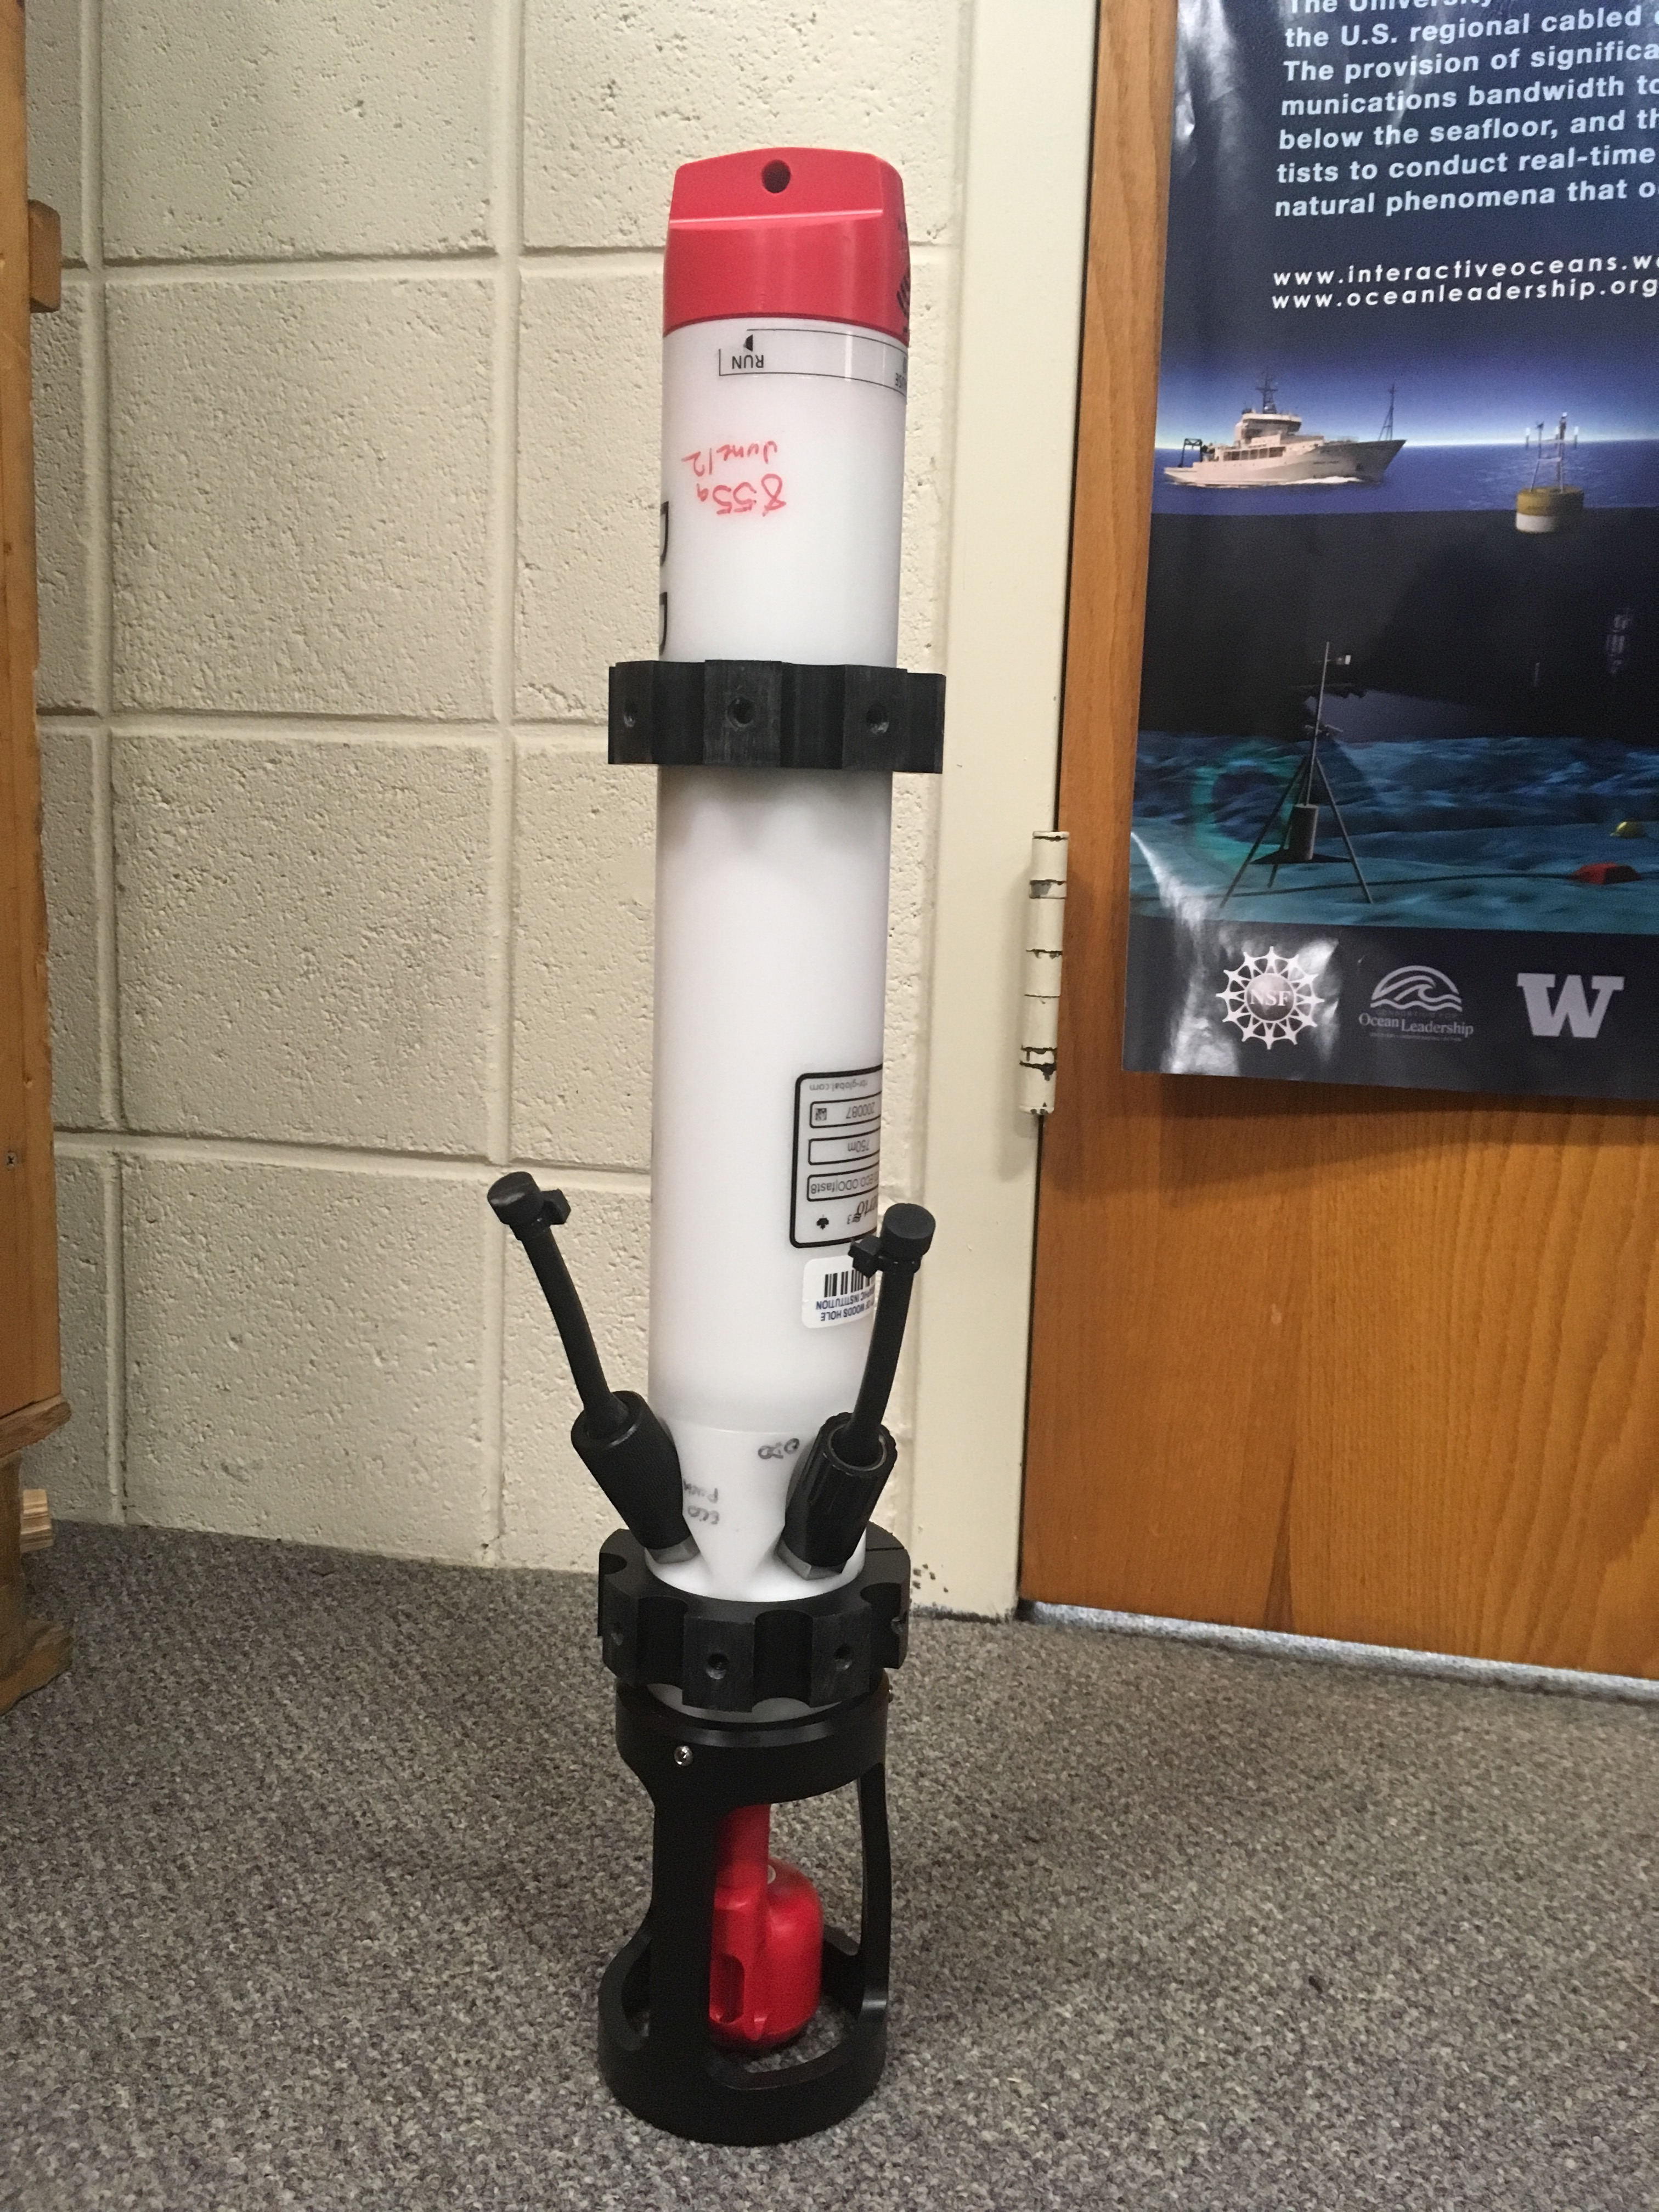
\includegraphics[width = 0.5\textwidth]{IMG_1640.JPG}
    \caption{CTD and logger with both clamps and guard attached}
    \label{fig:assemble2}
\end{figure}
        \item Tighten the clamps as much as possible so that the housing can slip over. The housing will fit very snugly but it should be able to slide over without using tools to force it down. At this stage, you may want to test that the clamps are properly aligned by fastening the housing. However, the housing will not be tightened until after the next step.
    \end{enumerate}
    \item Attach the cables to the external ports and run them upwards through the grooves in the clamps. Make sure you spend time giving some thoughts to where your cable will run. The end-cap of the CTD should be able to freely rotate 90 degrees, with no cables in the way. No cables should have to do a tight bend (Figure \ref{fig:assemble3})
    \begin{enumerate}
        \item The ODO cable is very long and needs to be wrapped twice. It is labeled ``interconnect straight through cable''
        \item The ECOPuck cable is short and should be run straight upwards from the external port. 
    \end{enumerate}
    \begin{figure}
        \centering
        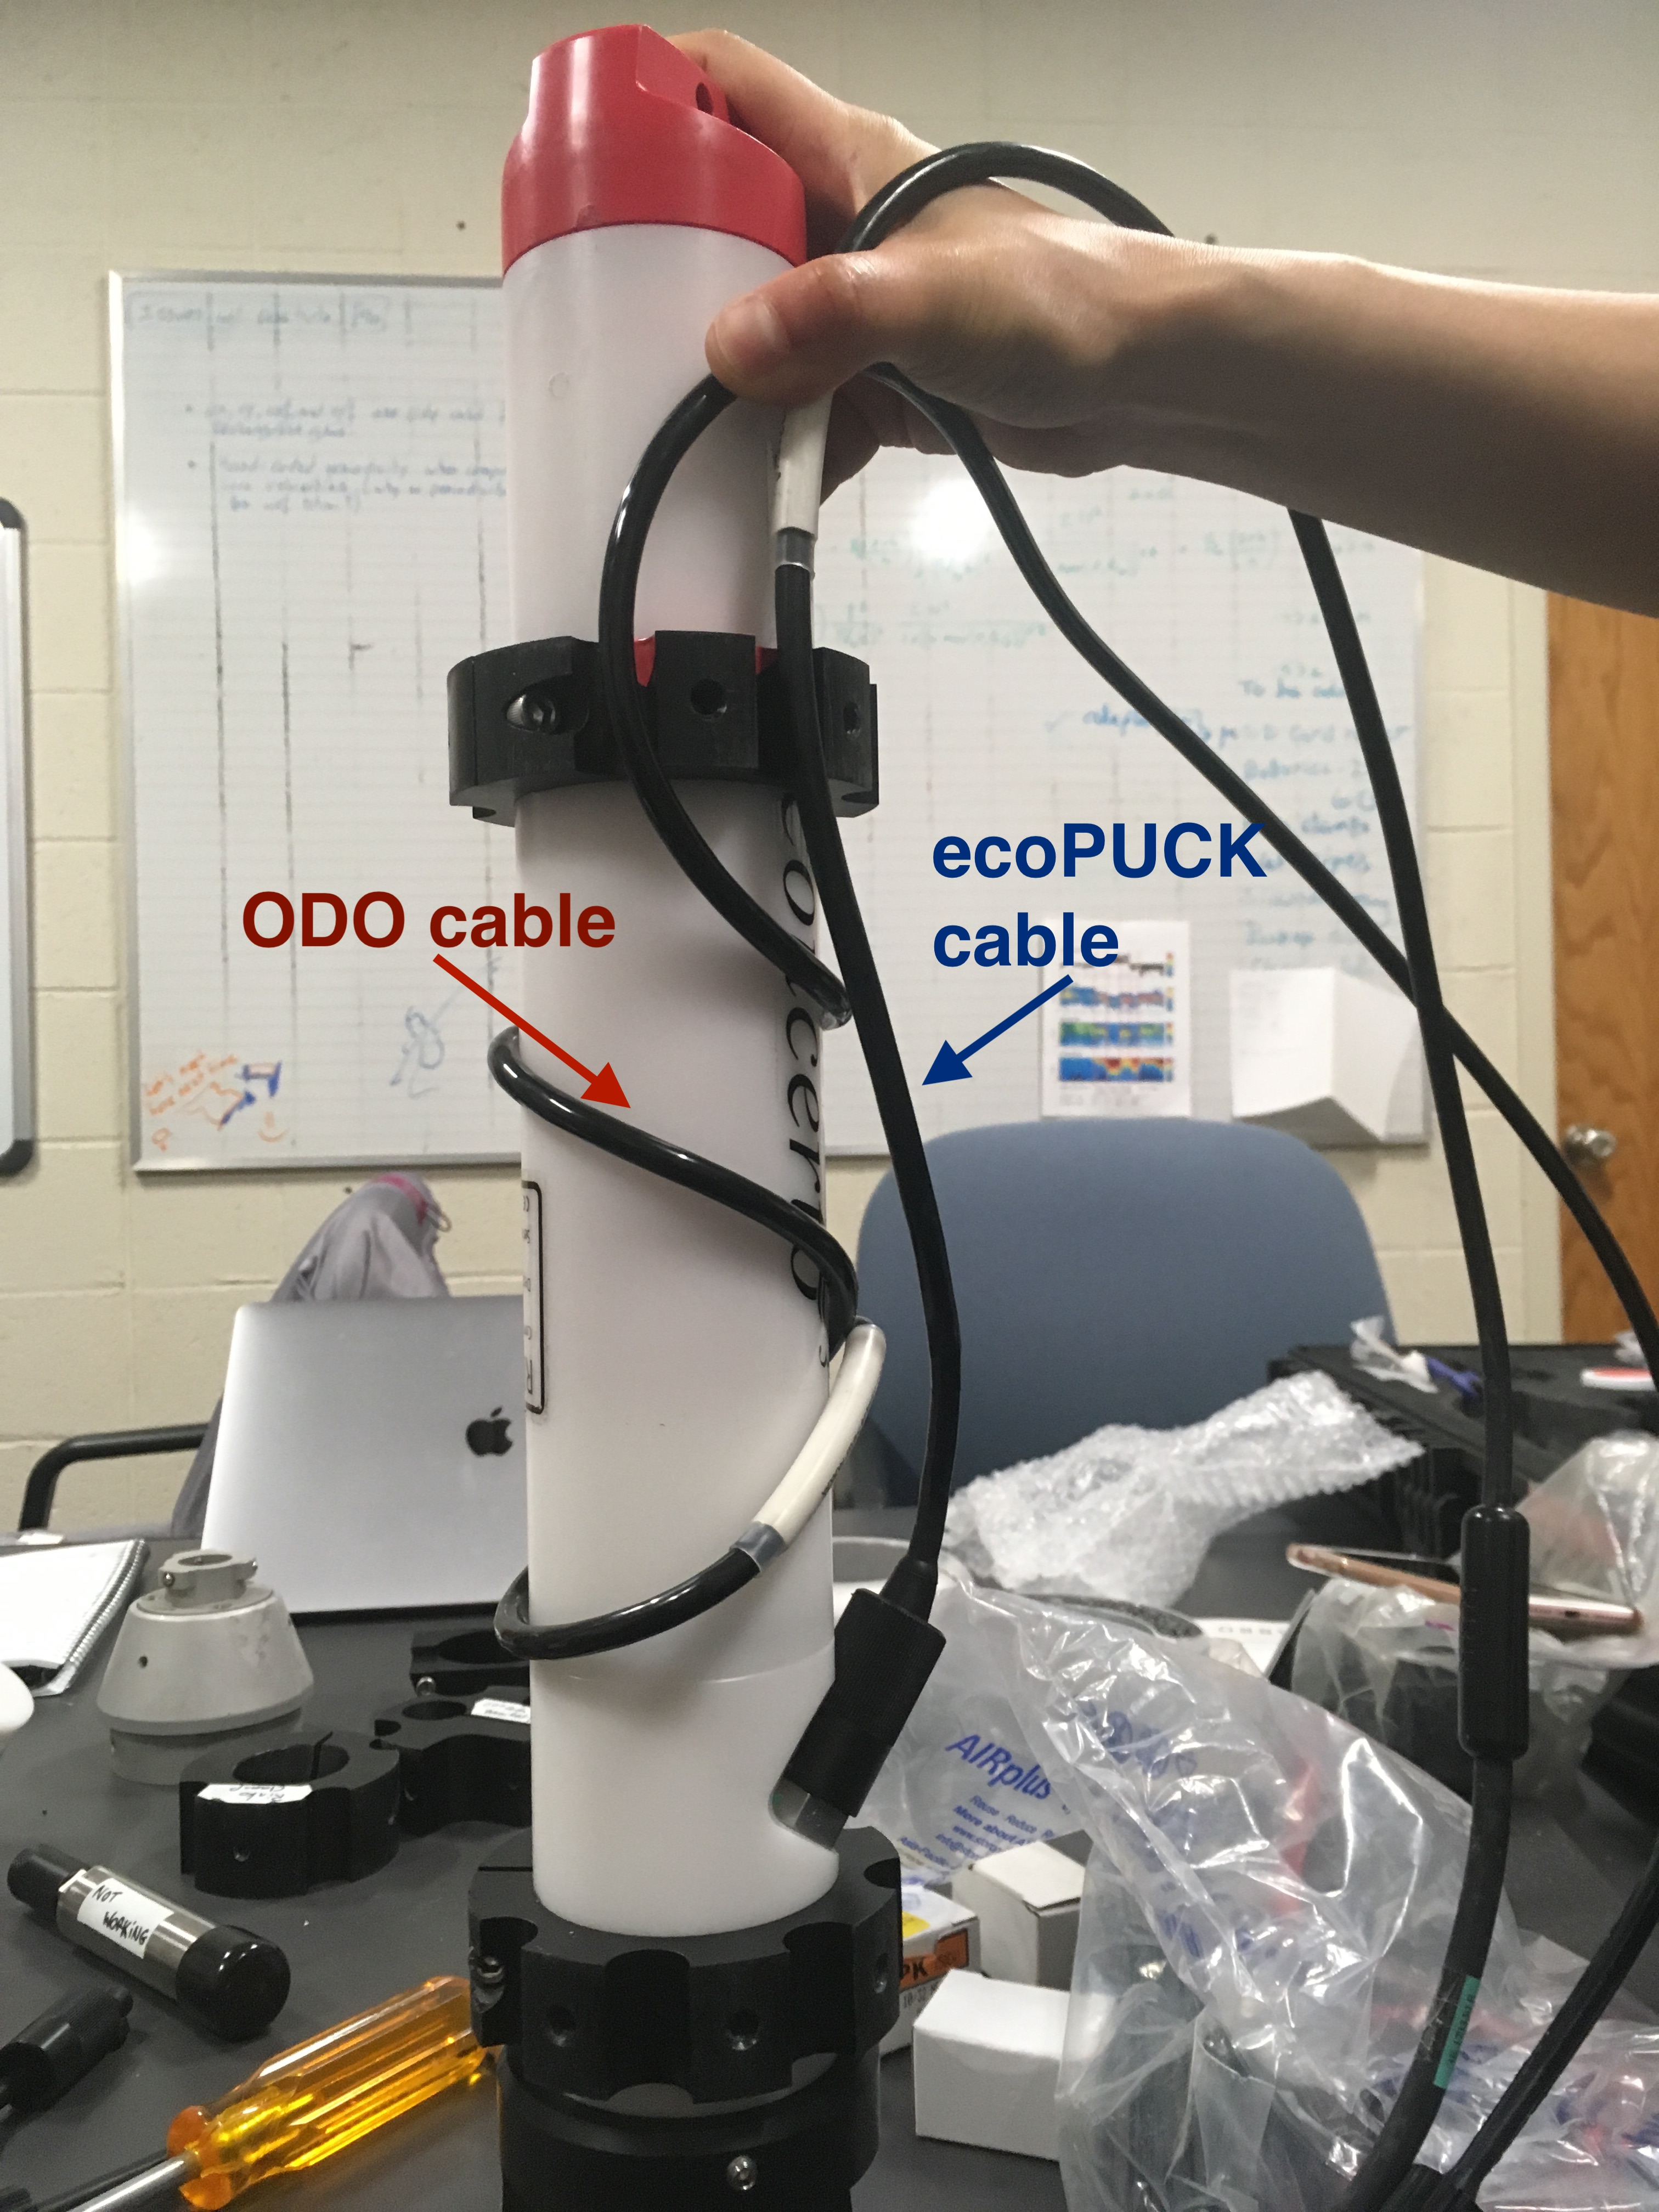
\includegraphics[width = 0.5\textwidth]{IMG_1642.JPG}
        \caption{Arrangement of cables}
        \label{fig:assemble3}
    \end{figure}
    \item Slide the lower housing over the logger. The cables should come upwards. Fasten the the lower housing with screws. Although there are four holes in the casing, only three screws are used. Every screw should have ``Aquashield" applied to it prior to being screwed in (Figure \ref{fig:assemble4}).
    \begin{figure}
        \centering
        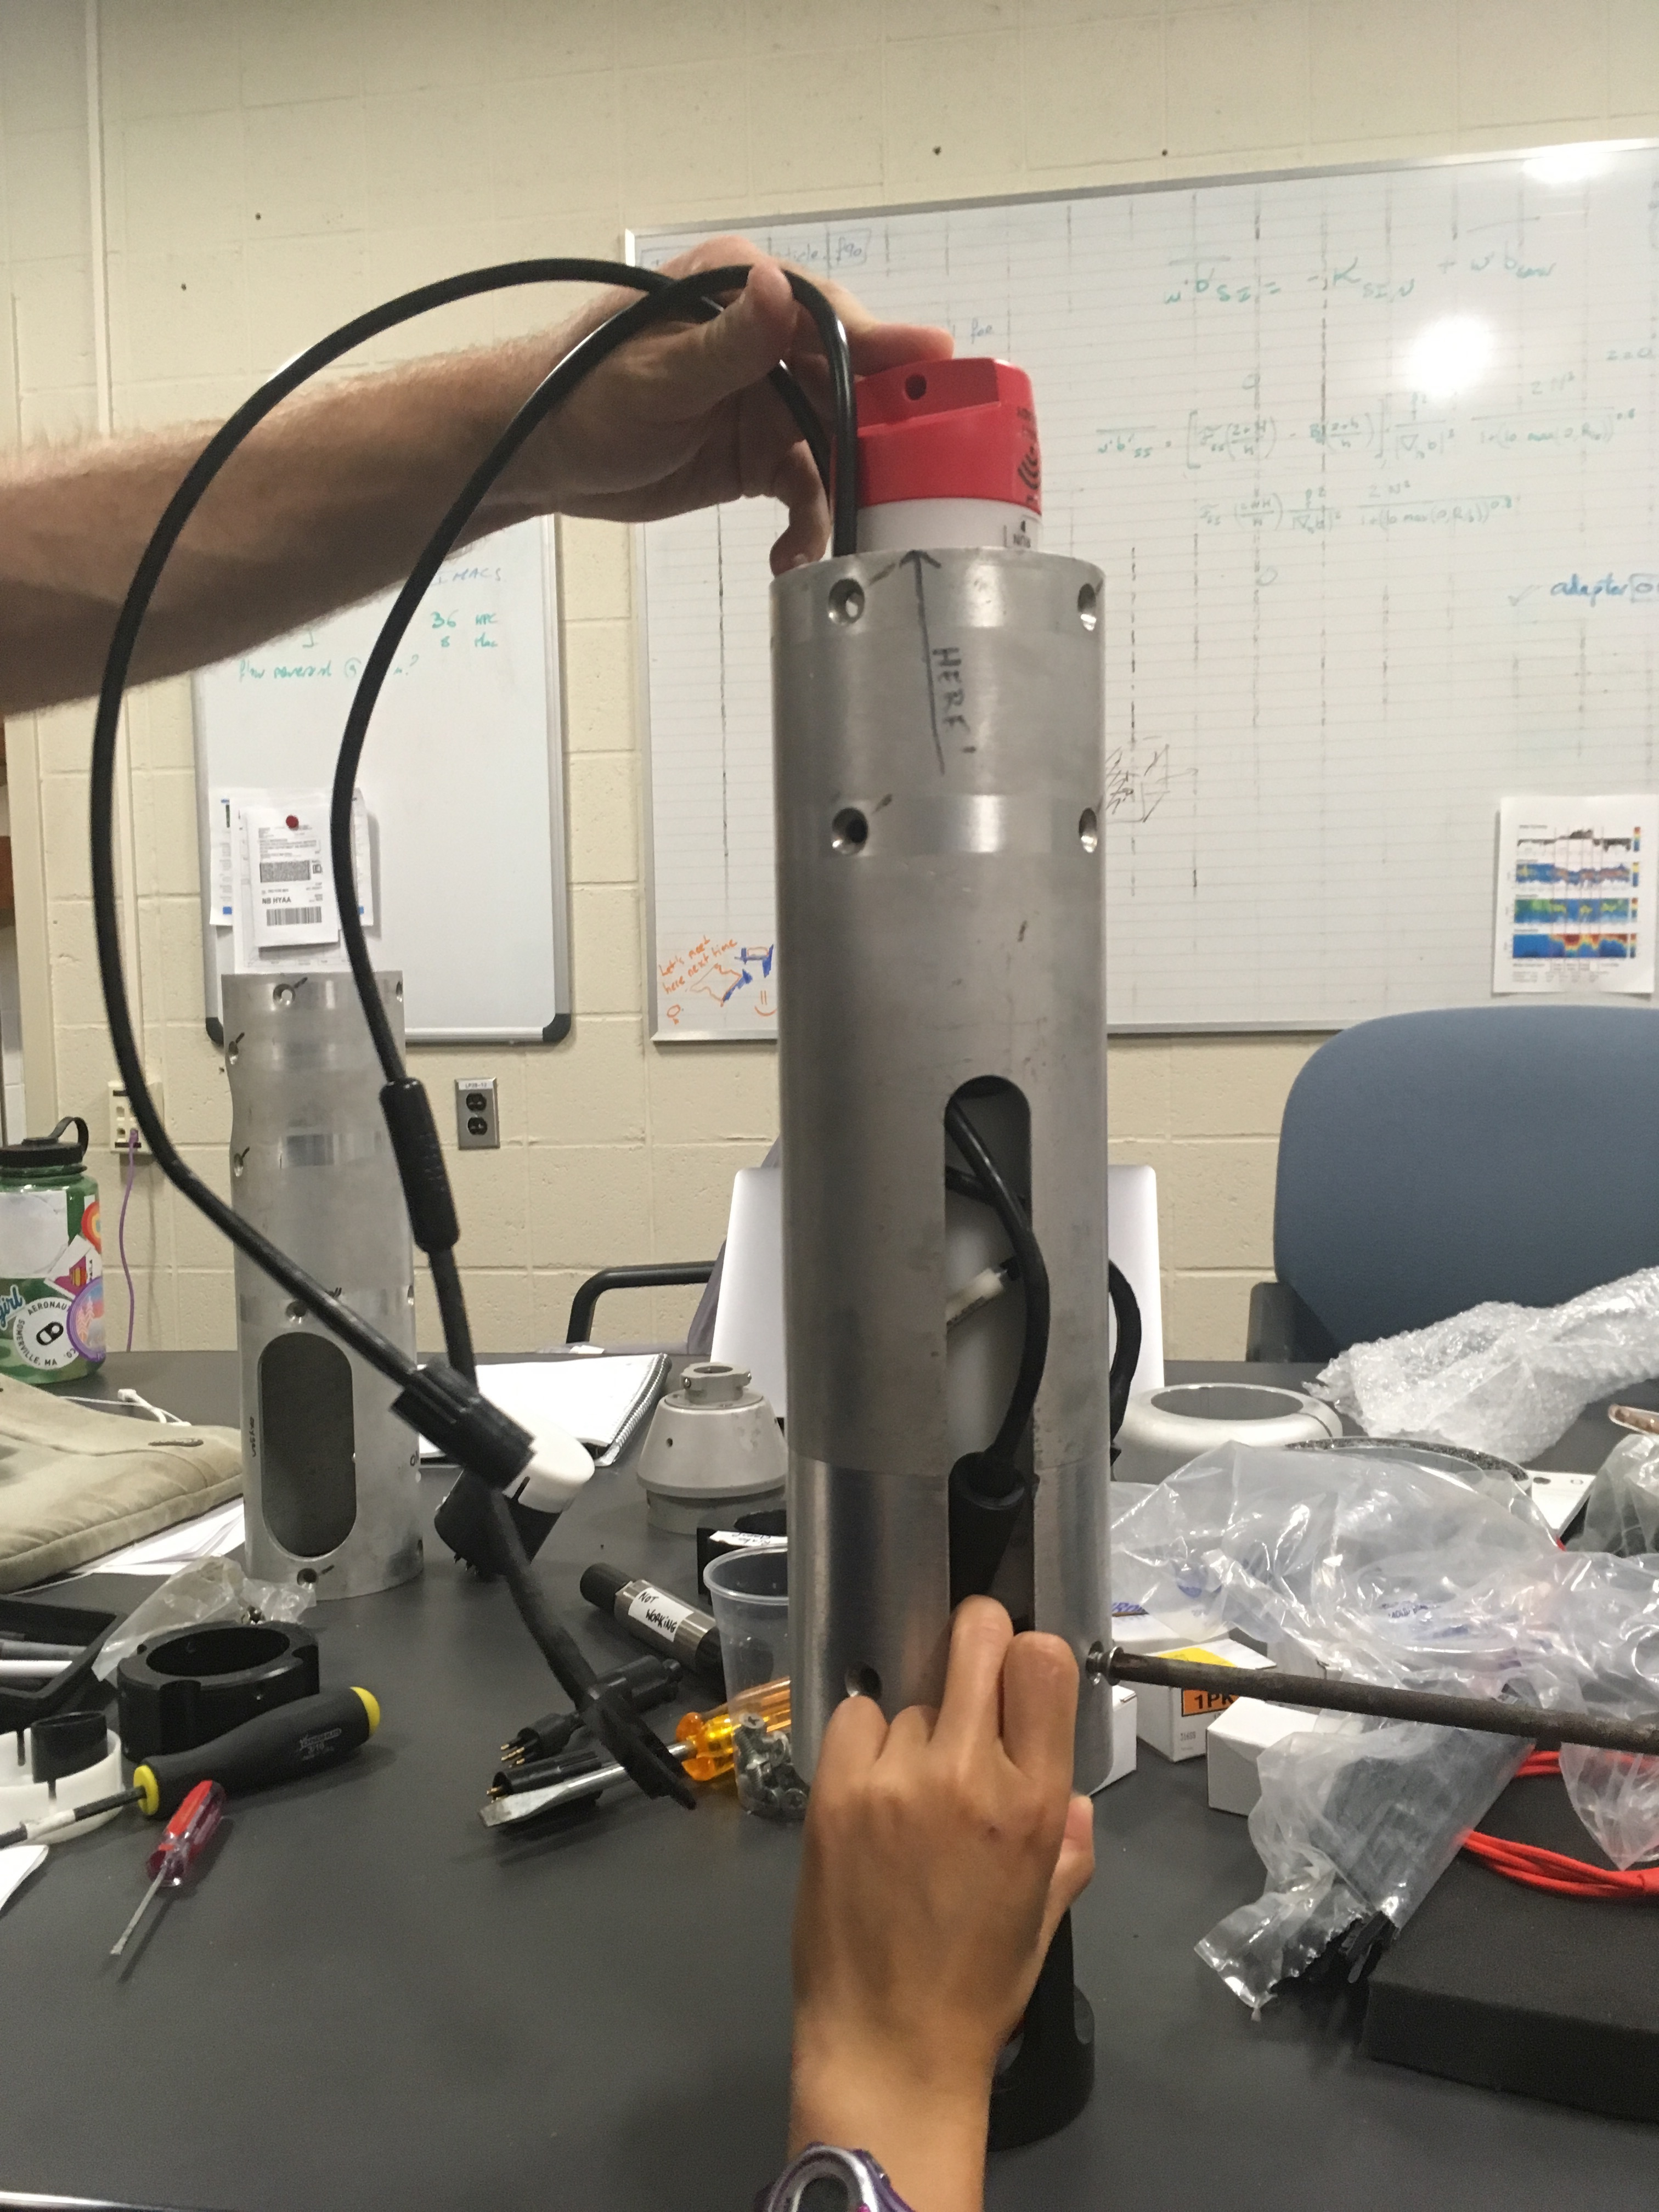
\includegraphics[width = 0.5\textwidth]{IMG_1643.JPG}
        \caption{Fastening lower housing}
        \label{fig:assemble4}
    \end{figure}
    \item Insert the union clamp into the top of the lower housing and screw it in. When you insert the union clamp, be mindful of the paths of the cables through the union clamp.
    \item Change the O-ring, put batteries in, and enable the logger before adding the upper housing ... having to disassemble/re-assemble may make you angry.
    \item Add the upper housing and screw into the union clamp. At this stage, ensure that the logger can be turned on and off through the slot in the upper housing (Figure \ref{fig:assemble5}).
    \begin{figure}
        \centering
        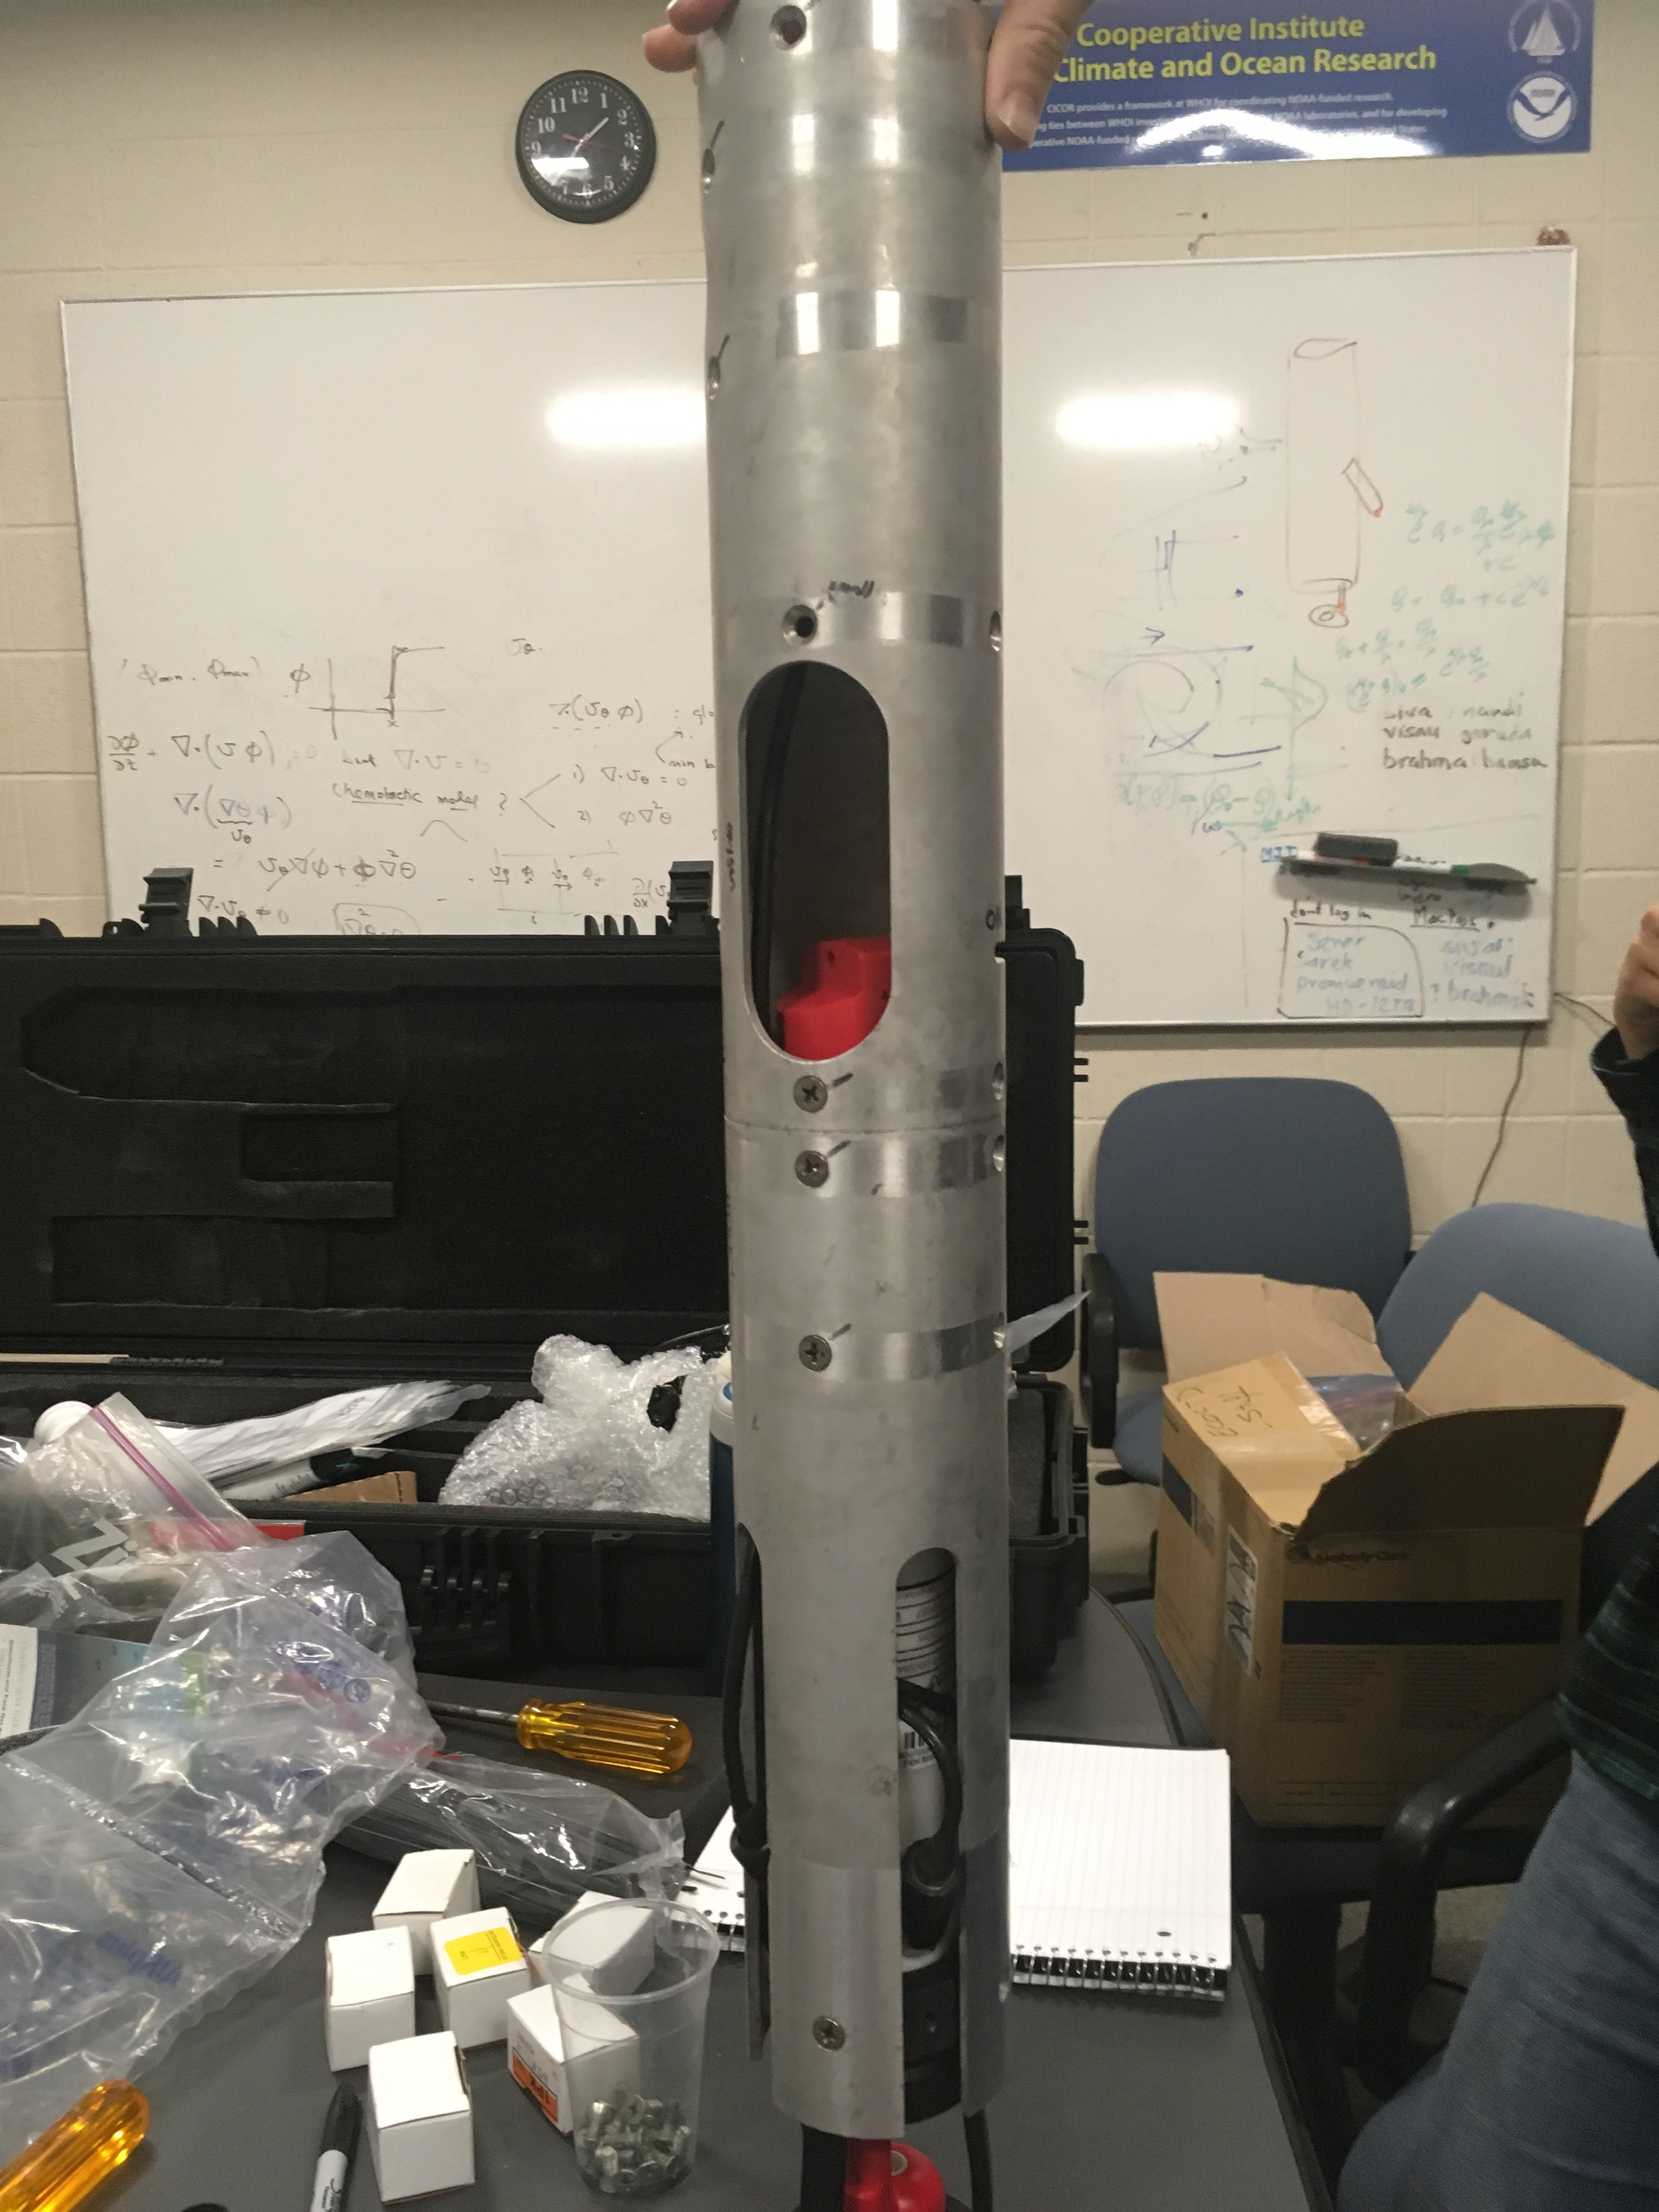
\includegraphics[width = 0.5\textwidth]{IMG_1644.JPG}
        \caption{Instrument with upper housing}
        \label{fig:assemble5}
    \end{figure}
    \begin{figure}
        \centering
        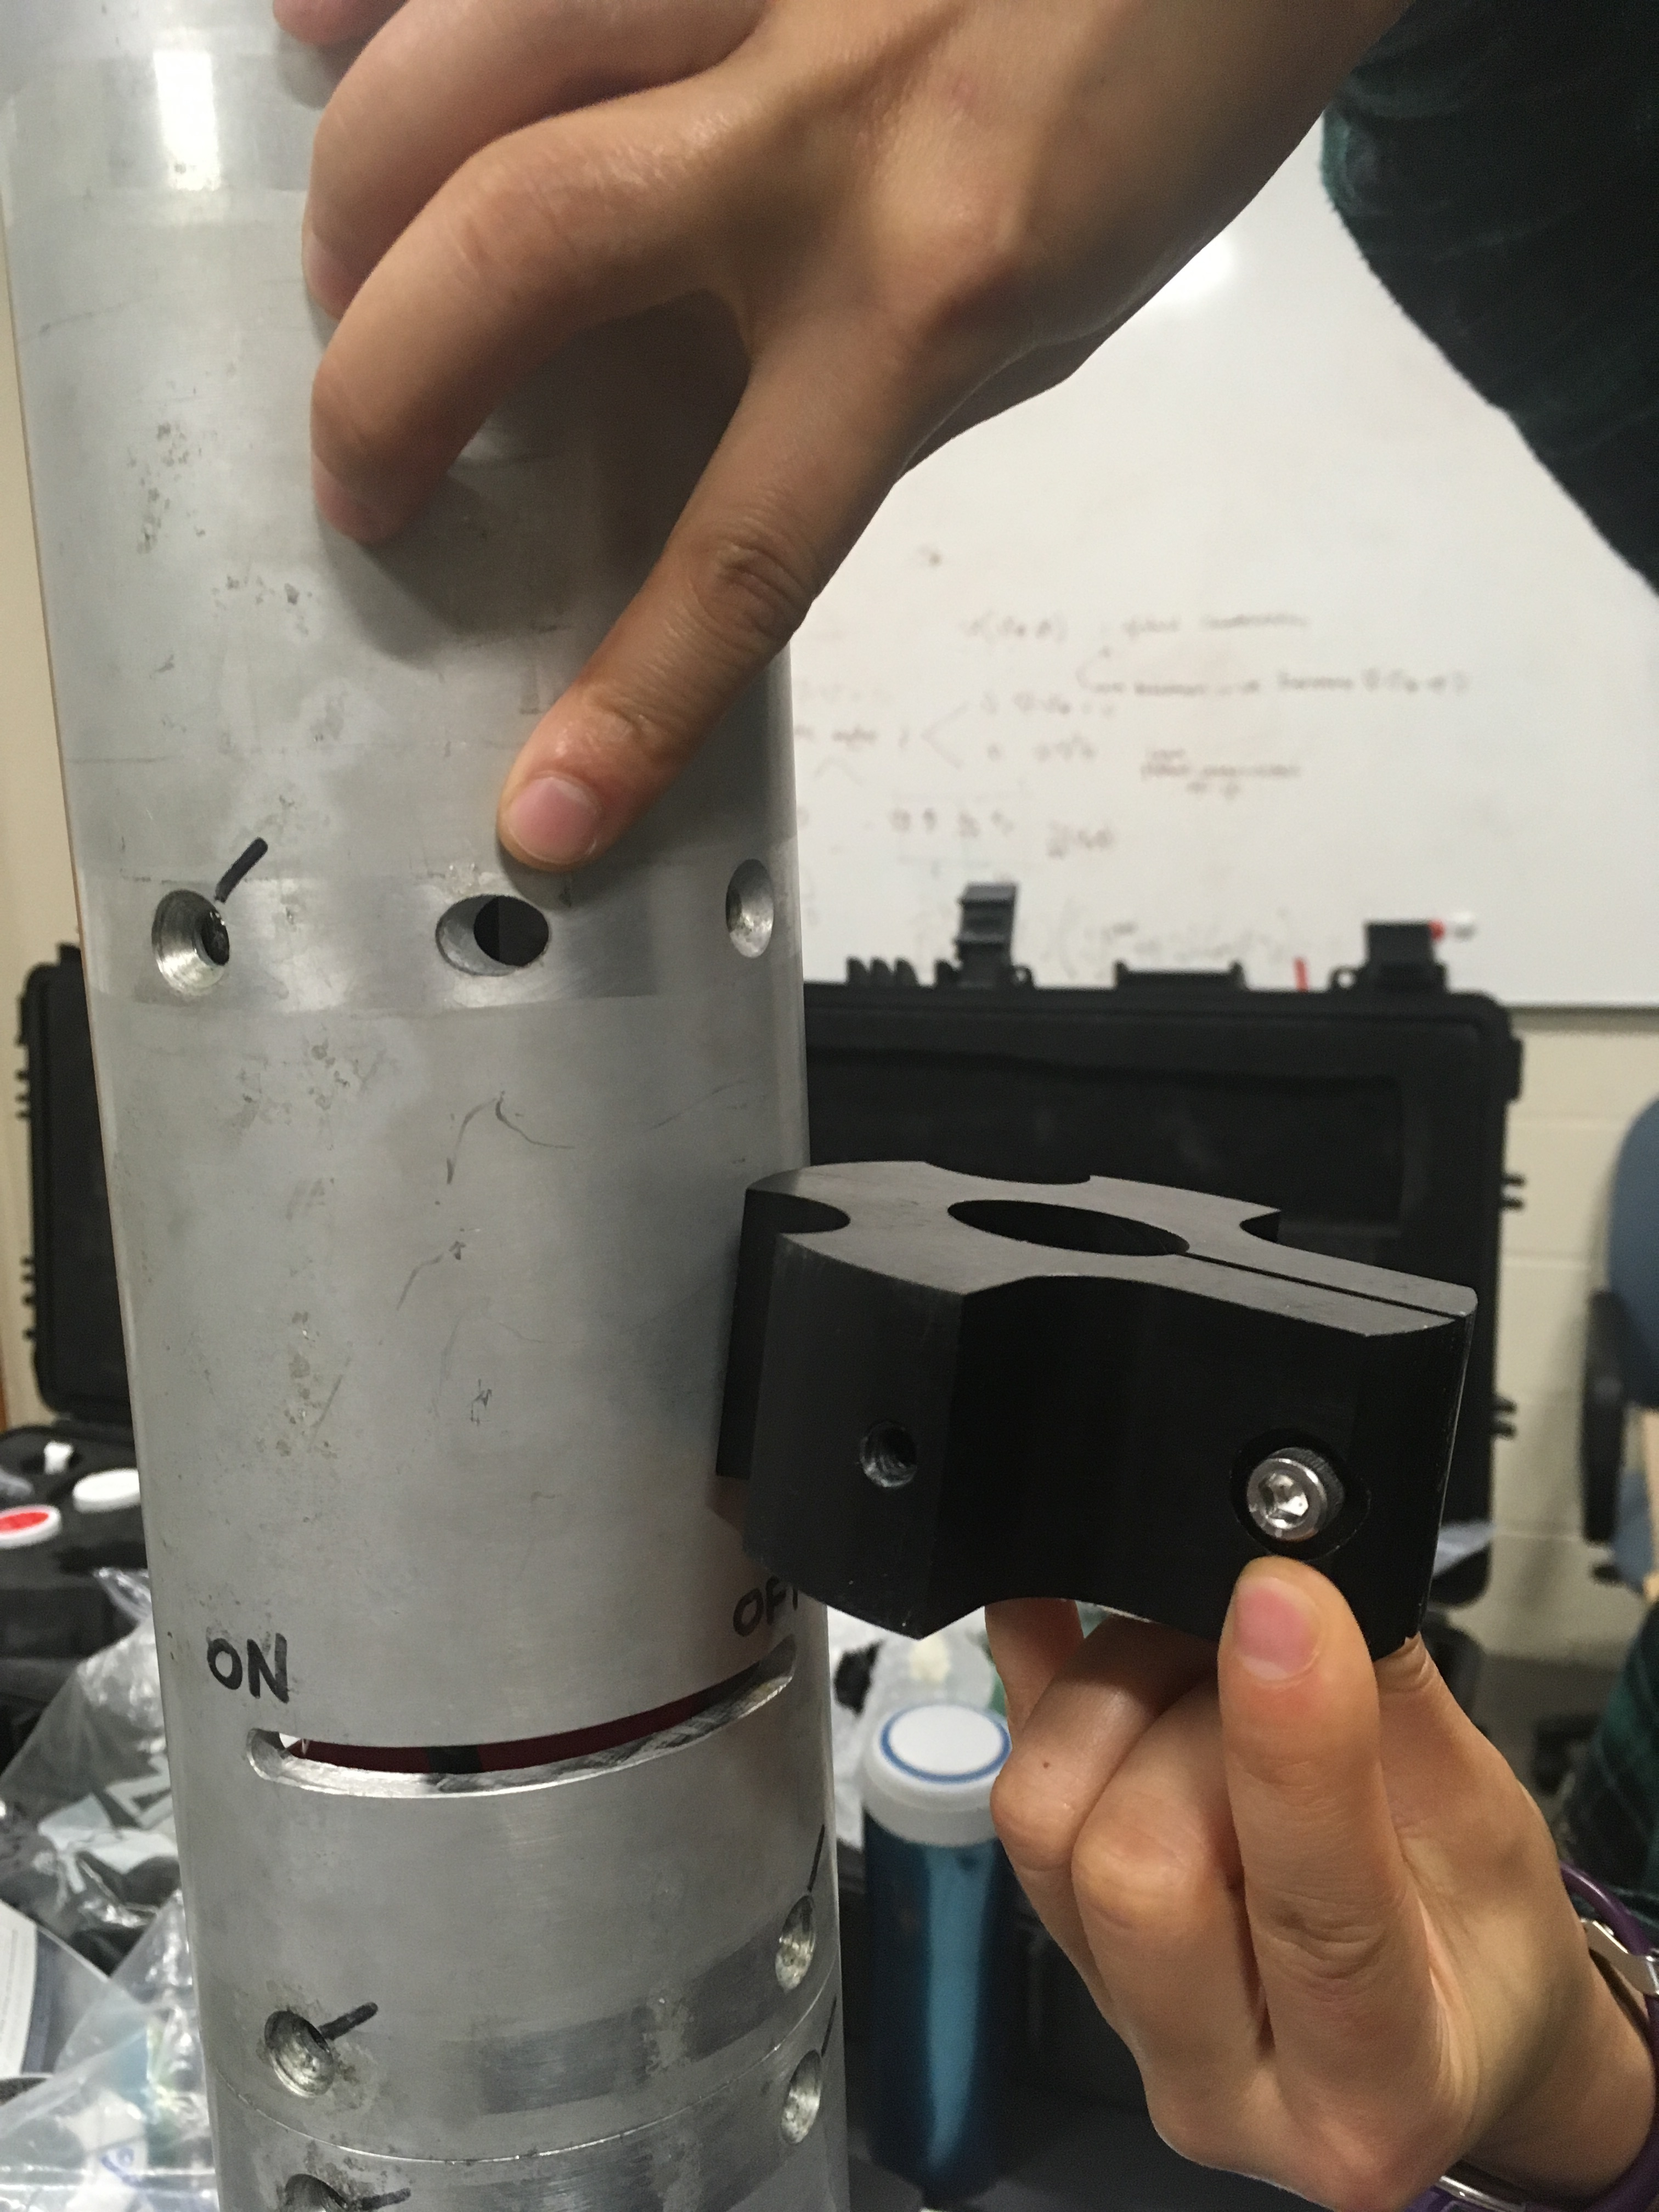
\includegraphics[width = 0.4\textwidth]{IMG_1645.JPG}
        \caption{Slanted screw hole and screw to which it corresponds}
        \label{fig:assemble6}
    \end{figure}
    \item Insert the oxygen sensor clamp into the upper housing. There is a slanted screw hole for the screw that tightens the oxygen sensor clamp around the oxygen sensor (Figure \ref{fig:assemble6}). Plug the oxygen sensor into the cable and insert from the outside. The oxygen sensor should be securely in the clamp, but should be far enough away from the instrument so as to be sampling undisturbed water. The oxygen sensor points downwards. The oxygen sensor clamp is then fastened to the upper housing.
    \item Insert the lower ECOPuck clamp. Fasten it to the upper housing with screws. Put the ECOPuck cable out of the instrument through the ECOPuck hole. Plug in the ECOPuck and rest on the lower ECOPuck clamp. Insert the upper ECOPuck clamp and tighten. 
    \item Pay extra attention to the UCTD coupling piece (TOP SPOOL BASE in diagram below) - this is what links the probe to the winch... make sure the screws and bolts are tight!
    \item Fasten the top spool base onto the upper housing. 
    \item Wrap the screws with electrical tape
    \item Attach the weight collar to the bottom of the lower housing. The weight collar abuts the cables.
    \item {\bf NOTE: } Every screw in the housing should have ``Aquashield" applied to it prior to being screwed in. It may be a good idea to only put one screw into each clamp during assembly in case parts need to be disassembled. 
\end{enumerate}

\begin{center}
    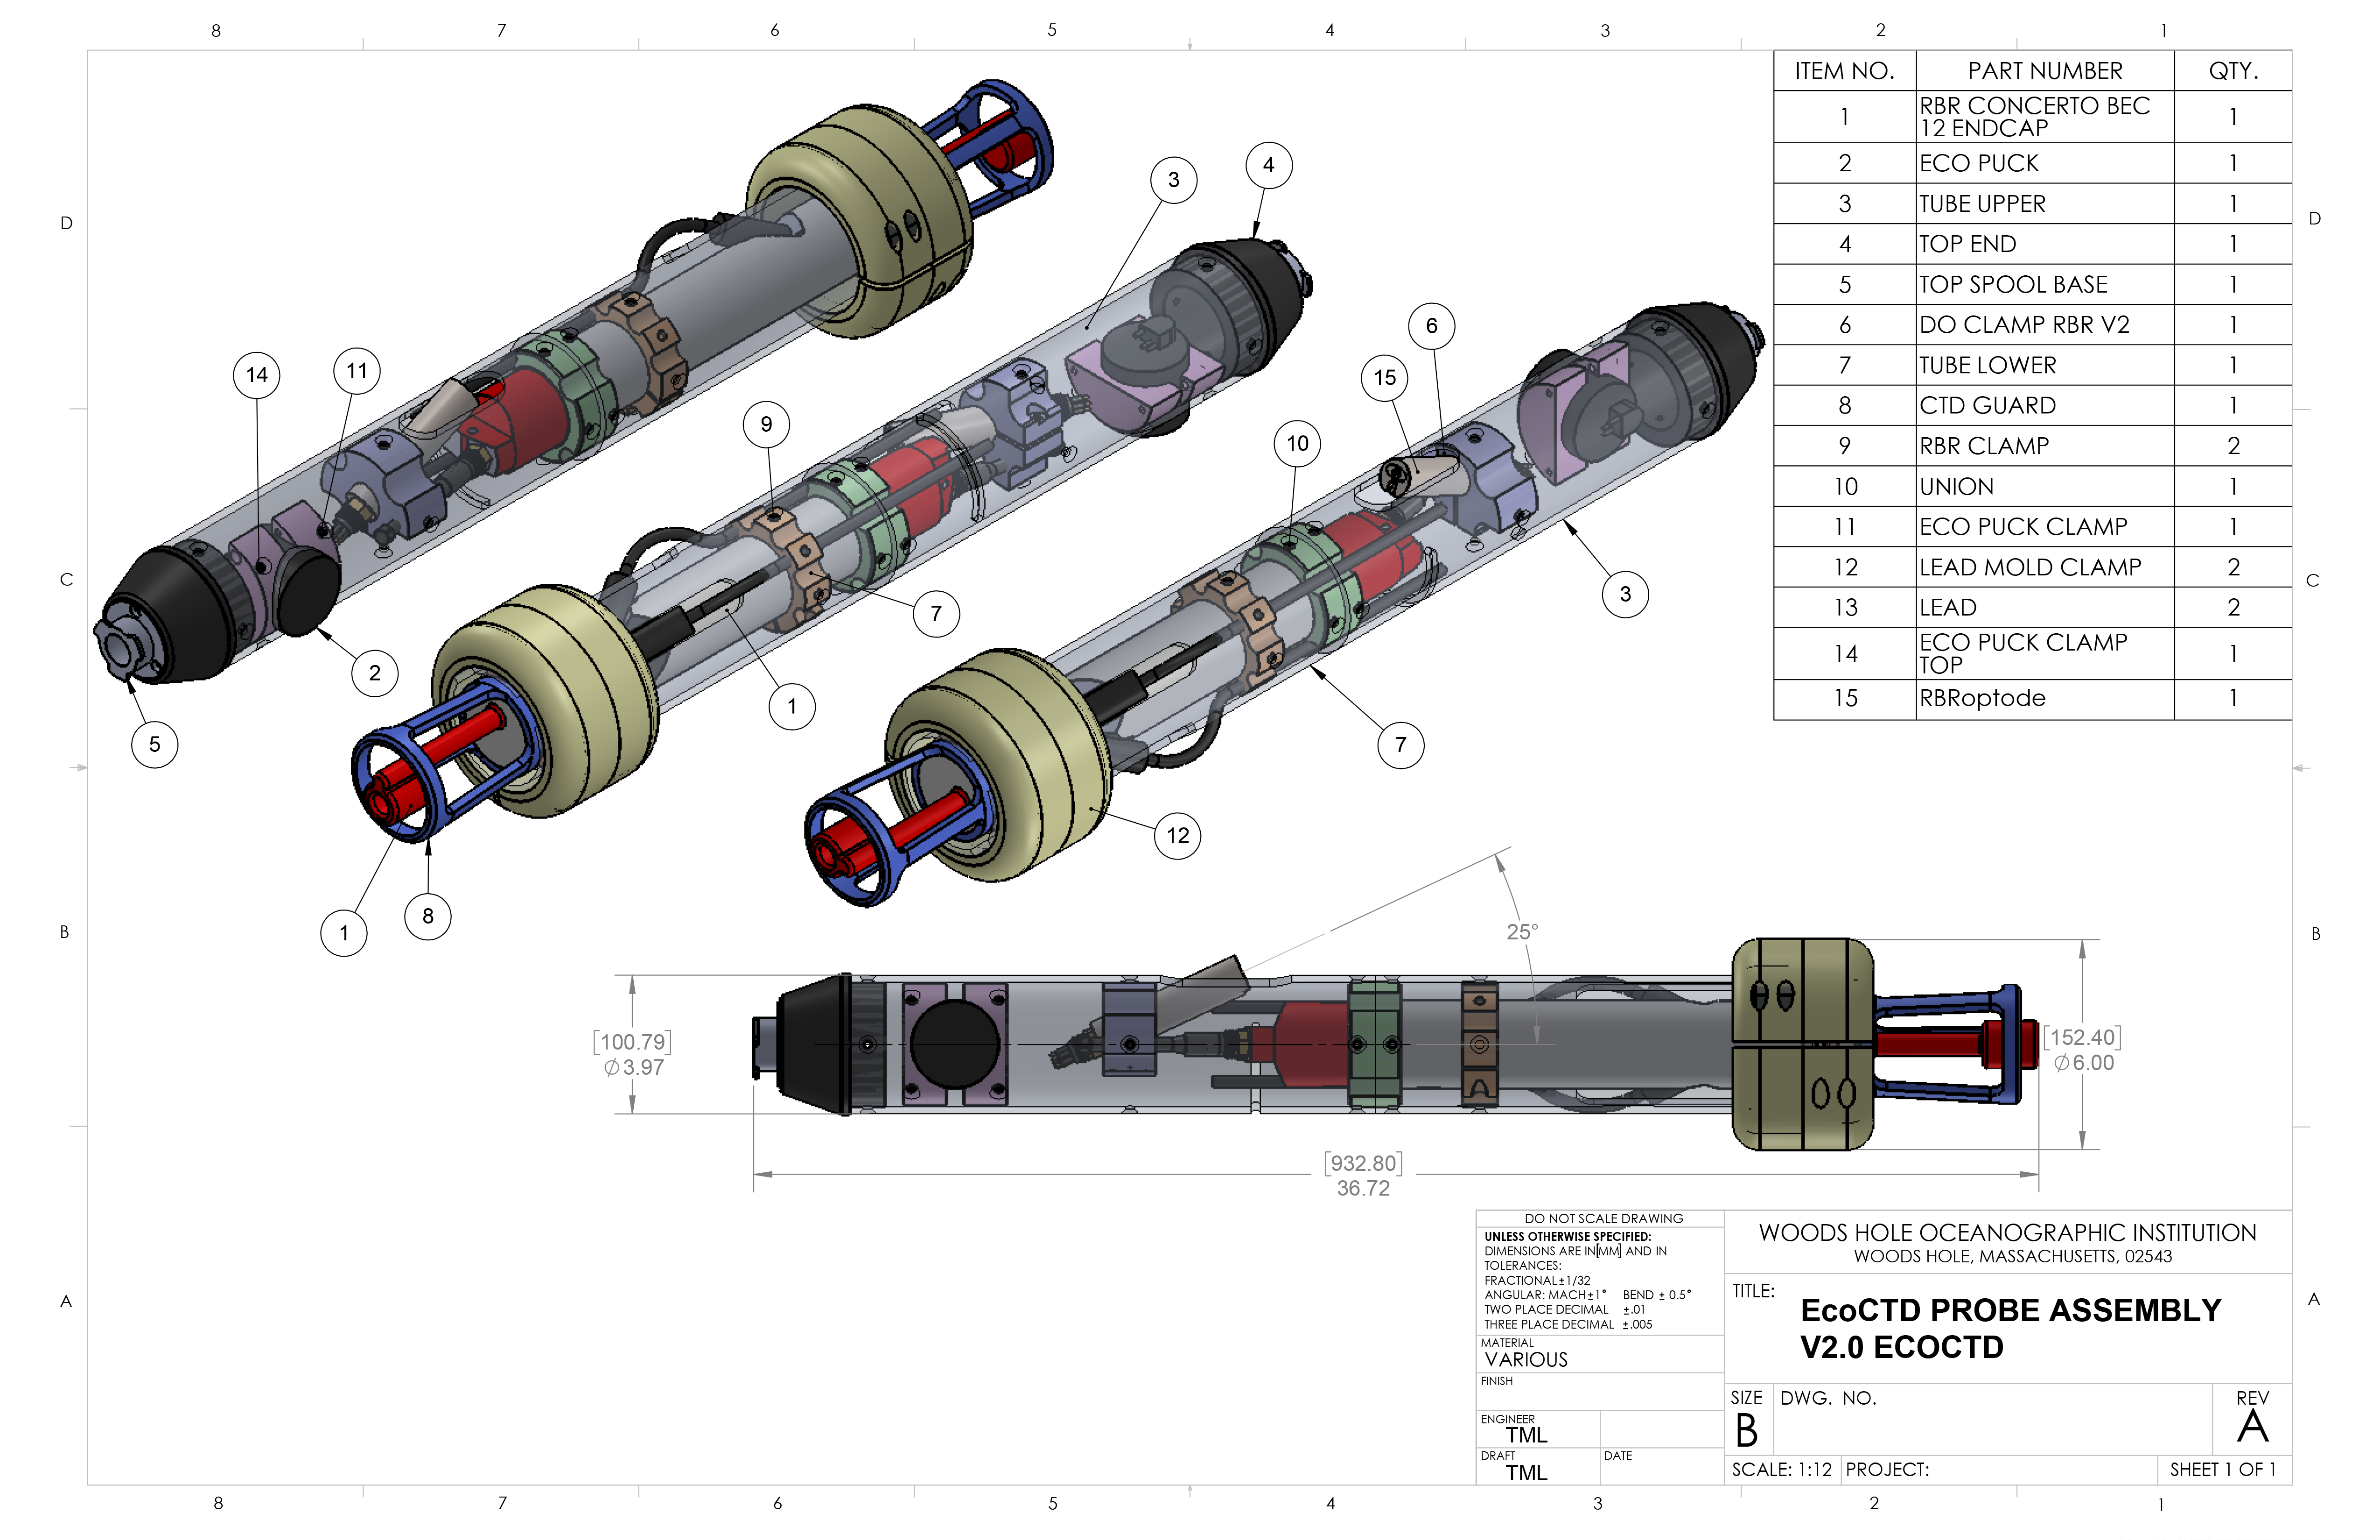
\includegraphics[width = .8\linewidth]{EcoCTD_engineer_diagram.png}
\end{center}

\subsection{Simulating EcoCTD in Ruskin}
To better predict the battery expectancy for a specific instrument, \ruskin has the ability to simulate an instrument setup. To do so, 
\begin{enumerate}
    \item click on the ``Instruments" menu, and then on ``Simulate Instrument..."
    \item Click on the ``Standard Instruments" tab
    \item 3 channels should already appear (conductivity, temperature, and pressure). Add a fourth channel corresponding to the EcoCTD setup. Likely, the EcoCTD will contain an oxygen sensor. Select ``Dissolved O2 concentration - RBRcoda T.ODO", as it corresponds to the oxygen sensor traditionally mounted on the EcoCTDs.
    \item To add the ECOPuck power consumption, you must add 3 additional channels labeled `Voltage"
    \item Select the option ``|fast8" in the bottom left corner. 
\end{enumerate}
By now, your screen should look like something like the image below. Note that Ruskin thinks it's a RBRmaestro, it's just because there's more channels than a typical RBRconcerto - you can ignore this.

\begin{center}
    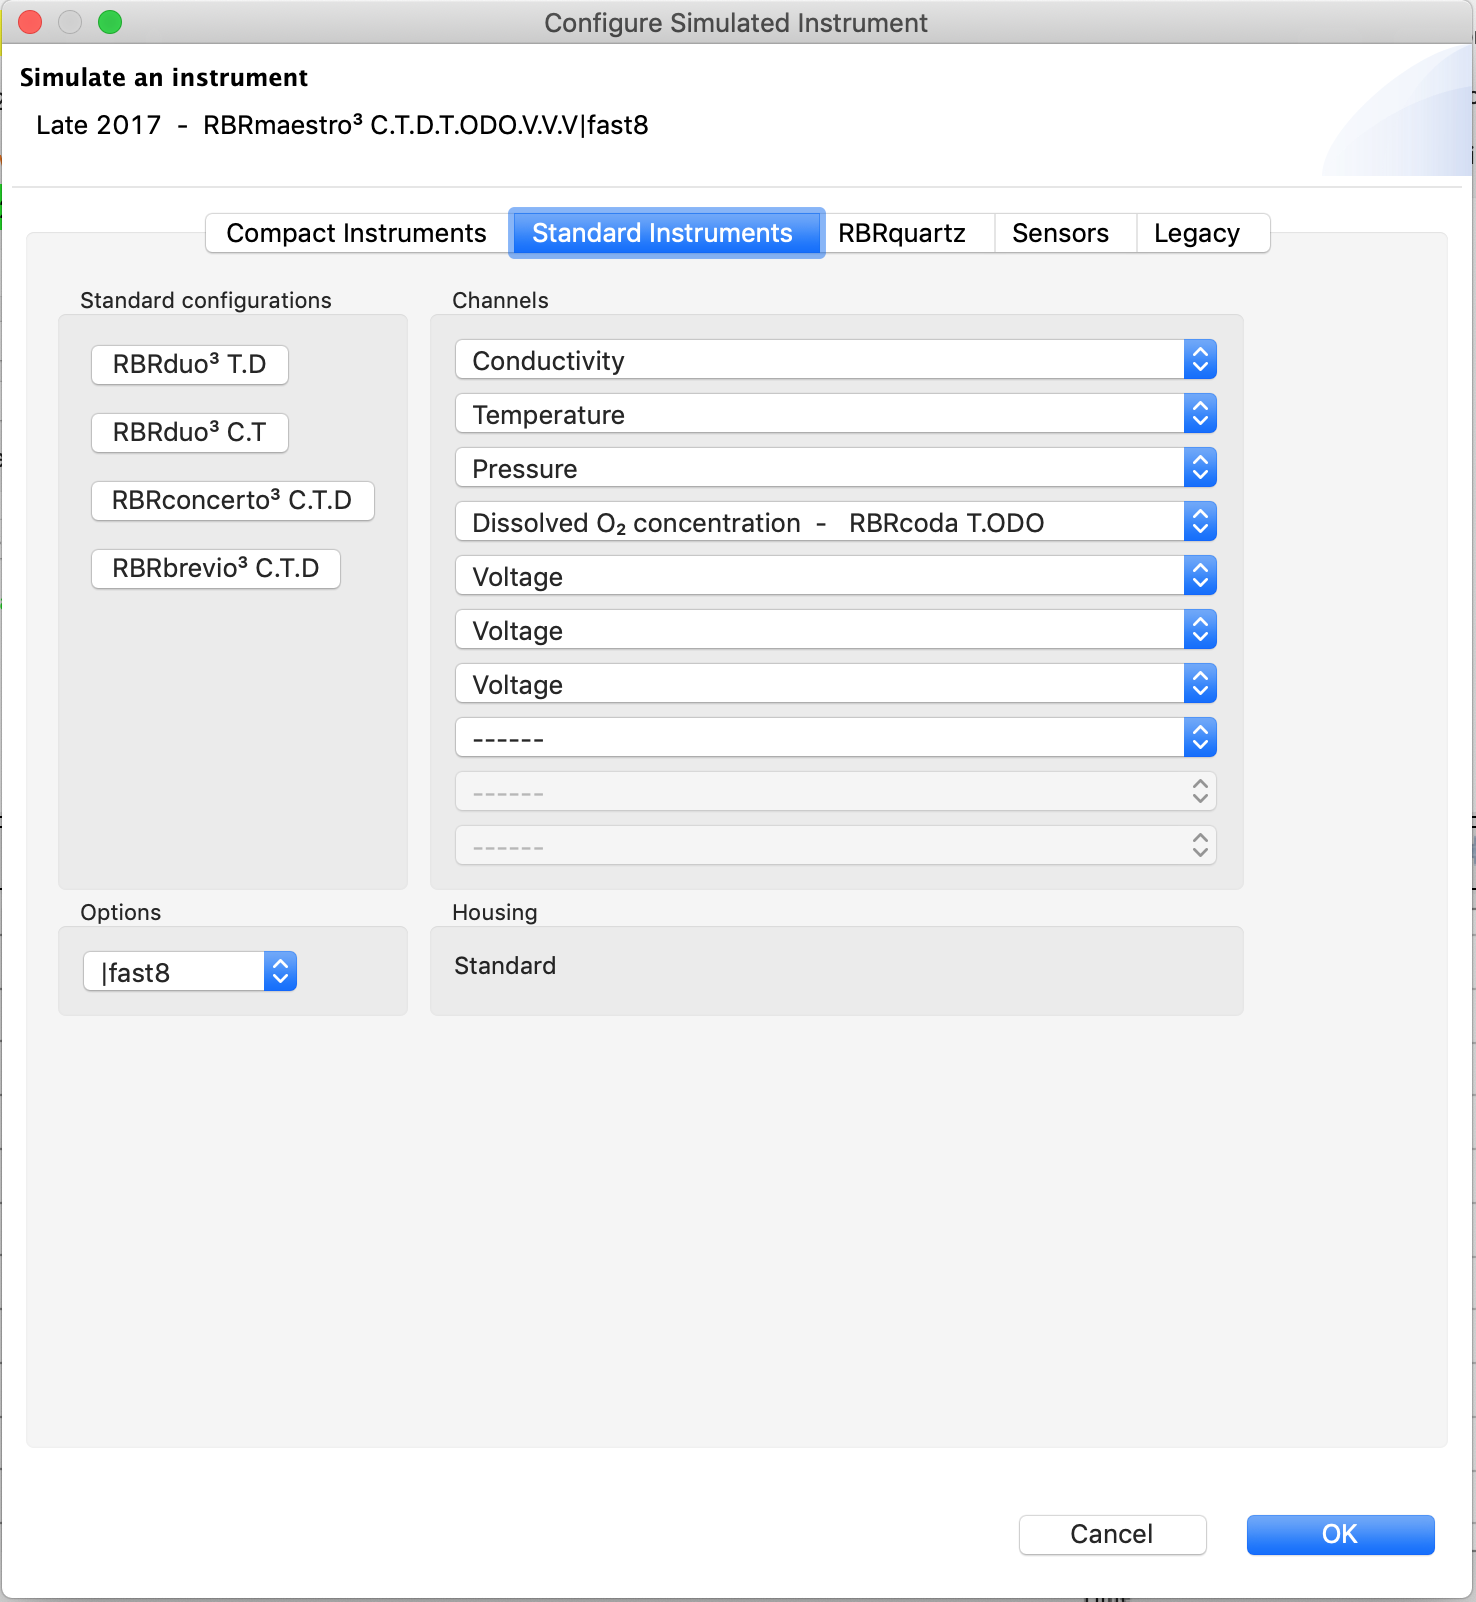
\includegraphics[width = .5\linewidth]{EcocTD_simulation.png}
\end{center}

\begin{enumerate}
    \item[6.]  On only \textbf{one} of the voltage channels, put in 1000ms for the Latency and 80mA for the Current. Leave the other 2 voltage channels with the default values. (see red square on image below)
    \item[7.] Select the type of battery that will be used to see the battery life expectancy in the bright green space located above the battery space.
    \item[8.] You can play around with the Sampling settings as well to see the battery life change, as well as storage life expectancy. In the case of the EcoCTD, the battery will always be the limiting factor before storage space.
\end{enumerate}

\begin{center}
    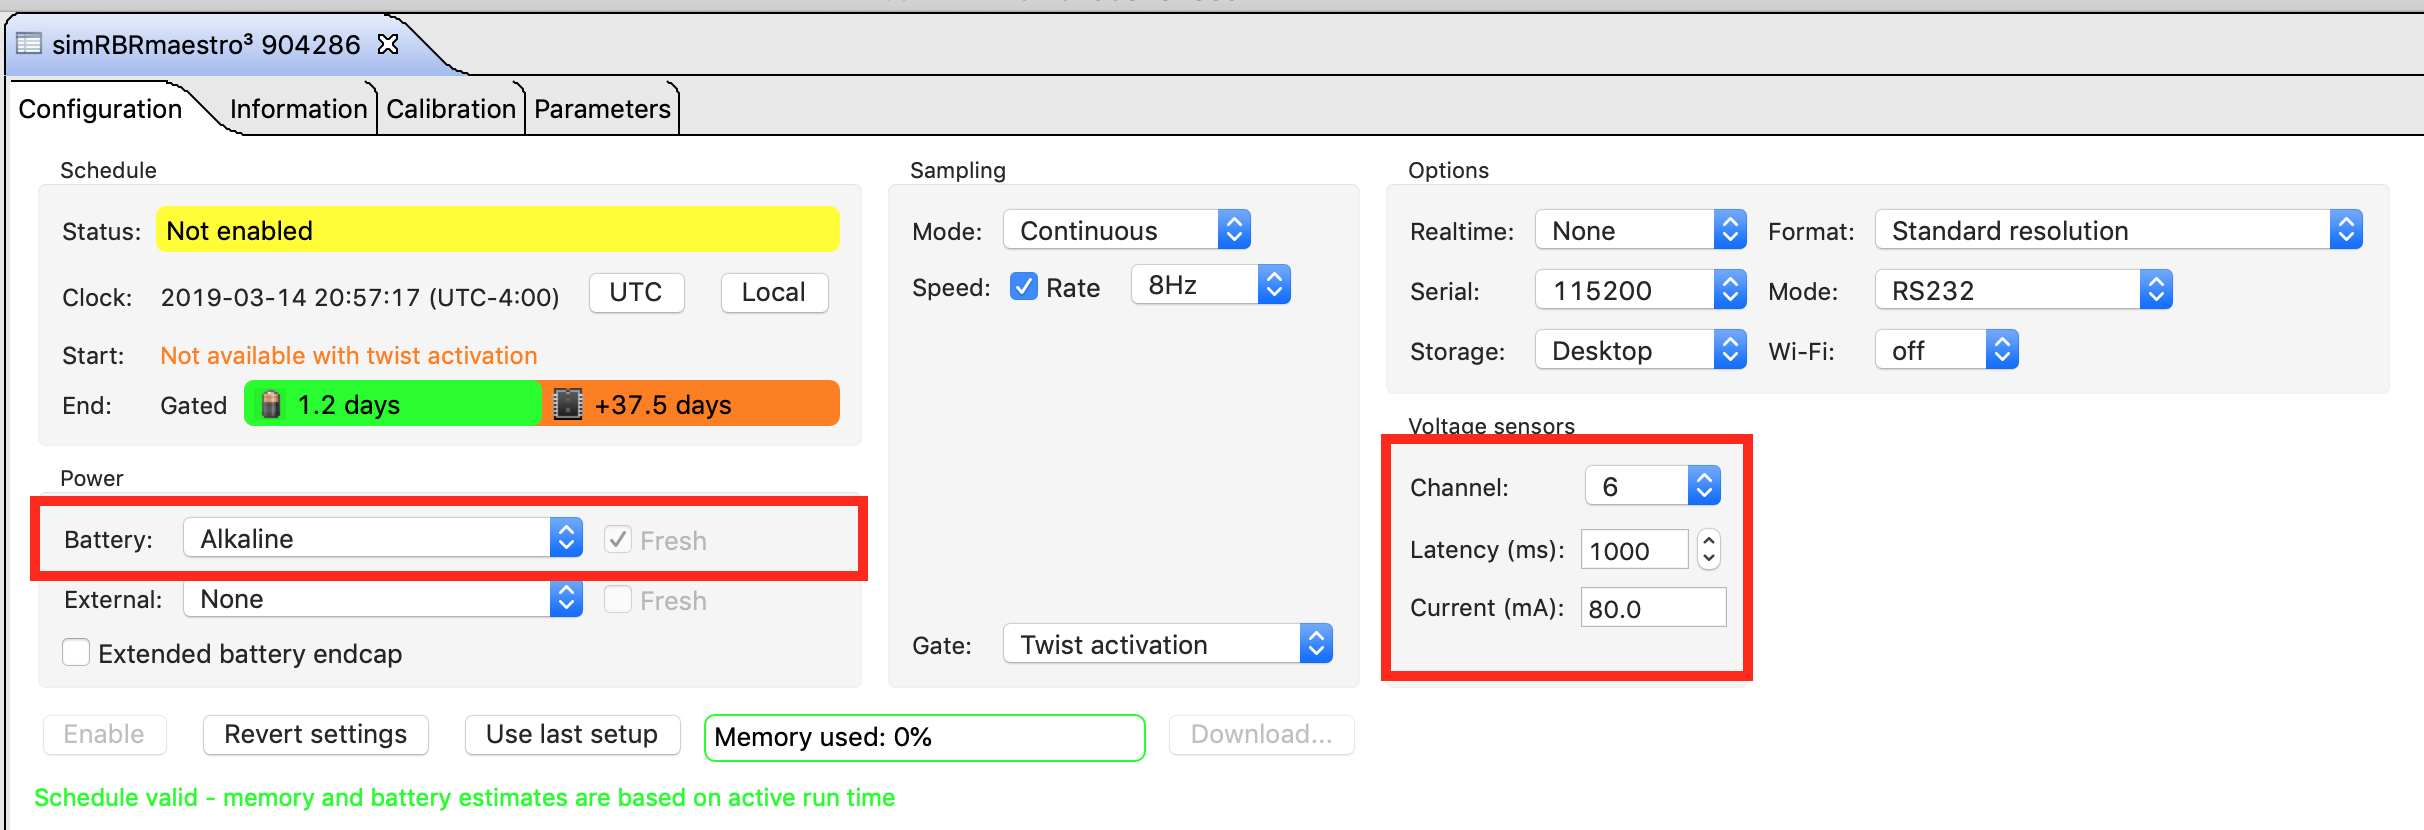
\includegraphics[width = .5\linewidth]{EcoCTD_simulation2.png}
\end{center}

\subsection{Configuring EcoCTD in Ruskin}
Most of what you need to know to configure the EcoCTD is in \ruskin's user manual. Traditionally, \begin{itemize}
    \item we sample continuously at 8Hz (we also use upcast for some variables), 
    \item we deactivate the Wi-Fi to save battery, 
    \item we use twist activation
\end{itemize}

\section{Deployment checklist}
Once the EcoCTD is configured, you can start thinking about deploying it. Here are the steps I usually followed:
\begin{enumerate}
    \item REMOVE all protective caps (oxygen sensor and ECOPuck if needed)
    \item Turn the instrument ON - you should see lights flashing on the ECOPuck. If you don't, you can go back to the work bench to troubleshoot.
    \item Connect the EcoCTD to the UCTD tail spool. \textbf{This part is important}. If the connection is not smooth (e.g., hard to rotate the tail spool, no clear clicking that says the tail is in place, constantly rotates without clicking), STOP what you are doing right now. There is a plastic screw in the tail spool that could be bent and taking the tail spool off might become a headache... or very easy. So if the EcoCTD is deployed this way, it might never come back.
    \item Engage the break on the UCTD winch. Slowly take the EcoCTD over the rail, and let it hang from the winch's davit.
    \item DO NOT drop the probe like it's done for the UCTD. The EcoCTD is not designed to hit the water at high speeds and sensors will be damaged. Instead, \textbf{GENTLY} lower the probe into the water until being dragged in the water 5-10 meters behind the ship. Be sure you give enough line so that a large wave trough would not suddenly make the EcoCTD airborn and fly into the stern of the ship... 
    \item release the break to start the profile. Don't forget to start your timer!! 
    \item {\color{red} The maximum depth rating is \textbf{500 m}- make sure you know how much time it corresponds to! drop rate is typically between 3.5 and 4 m/s so 2 minutes maximum should keep you on the safe side.}
\end{enumerate}

\section{Recovering the EcoCTD}
\textbf{Recovery can be tricky in rough weather.} Again, the principal danger is to go through a wave trough without enough line and have an EcoCTD swinging at full speed into the ship's stern. If you are not sure you are capable of safely retrieving the EcoCTD: (1) extend the UCTD winch davit to its maximum length, (2) use a pole to be able to push the line further outward and avoid collisions (but nothing with sharp edges that can cut the line, obviously!), (3) ask for help -- don't be a hero.

Once the EcoCTD is slowly, and vertically, being pulled up, have someone reach over the rail to carefully pull the probe in. Once on deck, place the protective caps back on. Disconnect the tail spool, paying attention to signs of wear (e.g., 360 degree rotating tail spool, hard to take off)

Finally, quickly wipe the EcoCTD with a rag. That minimizes chances of water entering the instrument, especially if the CTD needs to be opened for data download (see below).

\section{Data download}
Depending on which EcoCTD you use, you will have several options to download data, all of them require Ruskin.
\begin{itemize}
    \item if WiFi is enabled, you can download the data on your phone or computer. This is slow, unreliable, and battery consuming. Especially for larger datasets. It has been known to crop dataset without issuing warnings if the WiFi connection is momentarily lost. \textbf{This option is not recommended.}
    \item If connectorized end-cap (i.e., a cable comes out of the end-cap of the CTD), you can directly connect this to a USB port on a computer for data download. This is probably the easiest
    \item if regular endcap (EcoCTD v1.0 or ``Makara"), you need to take the four screws located at the bottom of the upper tube. The two tubes should be able to separate enough (if the cables were properly laid out during assembly, you should have enough slack) to reach the end-cap. Unscrew the end-cap and connect the USB cable. Make sure no water enters the instrument (shoule be fine if you dried the instrument after recovery as previously advised!).
    \item \textbf{Once data is downloaded, make sure you copy the RSK-file somewhere safe. Then copy it again somewhere else, also safe.}
    \item It is advised to wipe the memory of the logger after each data download. Data accumulates on the logger, and the subsequent download will get longer each time. You can wipe the memory by clicking the ``disable" button in Ruskin, and then the ``enable" button. It will issue a warning that memory will be wiped.
\end{itemize}

\section{Instrument maintenance}

\section{List of necessary supplies}


\end{document}
